\documentclass[utf8x]{beamer}
\usepackage[T1]{fontenc}
\usepackage{pgfpages}
\usepackage[czech]{babel}
\usepackage{lmodern}
\usepackage{tikz}
\usepackage{graphicx}
\usepackage{microtype}
\usepackage[outputdir=build]{minted}

\definecolor{vulkan}{HTML}{ac162c}
\hypersetup{colorlinks, urlcolor=vulkan}
\setbeamercolor{titlelike}{fg=vulkan}
\setbeamercolor{item}{fg=black}
\setbeamertemplate{navigation symbols}{}
\setbeamertemplate{caption}{\insertcaption}
\setbeamertemplate{note page}[plain]
\setbeamerfont{note page}{family=\rmfamily}
\setbeamerfont{title}{family=\rmfamily, size=\Huge}

\newcommand\blfootnote[1]{%
  \begingroup
  \renewcommand\thefootnote{}\footnote{#1}%
  \addtocounter{footnote}{-1}%
  \endgroup
}

% https://github.com/microsoft/dotnet/tree/master/releases/reference-assemblies
% 
% https://www.mono-project.com/docs/advanced/runtime/
% https://docs.microsoft.com/en-us/dotnet/standard/clr
% https://docs.microsoft.com/en-us/archive/msdn-magazine/2019/july/csharp-net-reunified-microsoft%E2%80%99s-plans-for-net-5
% https://www.youtube.com/watch?v=Jw88UYVG9dg
% https://github.com/microsoft/msbuild/issues/4751

\date{duben 2020}
\author{Adam Štěpánek}
\newcommand*{\at}{@}
\institute{\href{mailto:adam.stepanek\at riganti.cz}{adam.stepanek\at riganti.cz} \\
    \href{mailto:xstepan1\at fi.muni.cz}{xstepan1\at fi.muni.cz}}
\title{.NET na Linuxech}

\begin{document}

\begin{frame}
    \titlepage
\end{frame}
\note{}

\begin{frame}
    \begin{itemize}
        \item Motivace
        \item Víc než jeden .NET
        \item Instalace
        \item Vývojové prostředí
        \item Knihovny
        \item Problémy
        \item Jeden .NET
    \end{itemize}
\end{frame}

\begin{frame}
    \begin{center}
        \color{vulkan}
        \Huge \textrm{Motivace}
    \end{center}
\end{frame}

\begin{frame}
    \begin{center}
        \color{vulkan}
        \Huge \textrm{Víc než jeden .NET}
    \end{center}
\end{frame}

\newcommand{\tale}[1]{
    {
        \begin{frame}[plain]
            \centering
            \includegraphics[width=\textwidth]{#1}
        \end{frame}
    }
}

\tale{tale/01.png}
\tale{tale/02.png}
\tale{tale/03.png}
\tale{tale/04.png}
\tale{tale/05.png}

\begin{frame}[plain]
    \centering
    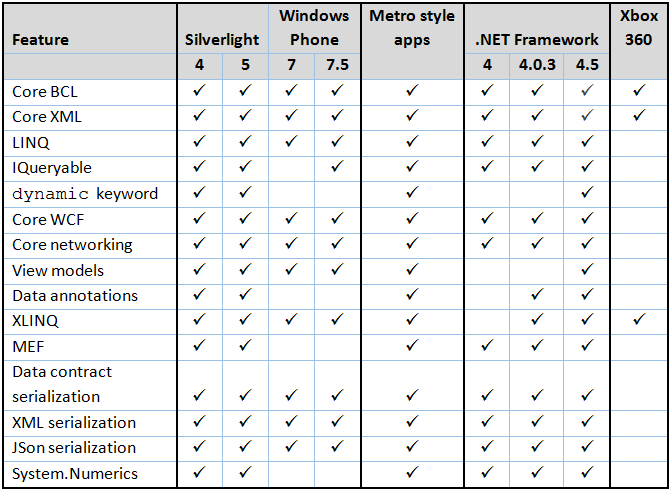
\includegraphics[width=\textwidth]{pcl.png}
    \tiny\url{https://docs.microsoft.com/en-us/archive/blogs/dsplaisted/how-to-make-portable-class-libraries-work-for-you}
\end{frame}

\tale{tale/06.png}
\tale{tale/07.png}
\tale{tale/08.png}
\tale{tale/09.png}
\tale{tale/11.png}
\tale{tale/12.png}
\tale{tale/13.png}

\begin{frame}[plain]
    \centering
    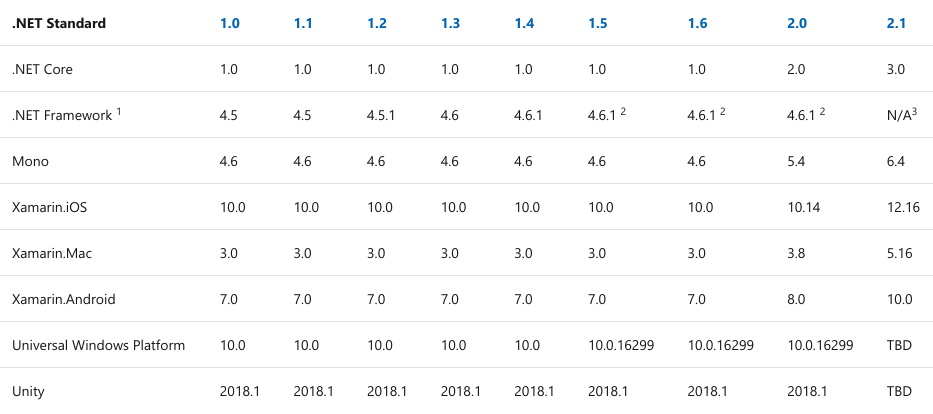
\includegraphics[width=\textwidth]{netstandard.png}
    \tiny\url{https://docs.microsoft.com/en-us/dotnet/standard/net-standard}
\end{frame}

\begin{frame}
    \begin{center}
        \color{vulkan}
        \Huge \textrm{Instalace}
    \end{center}
\end{frame}

\begin{frame}
    \centering
    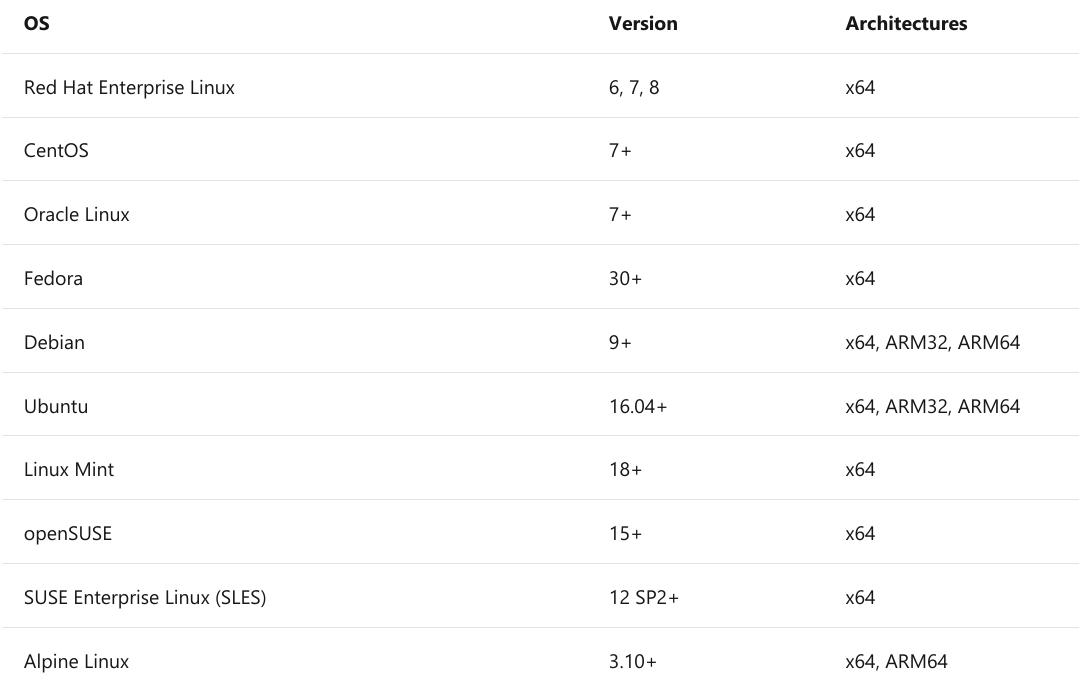
\includegraphics[width=\textwidth]{support.png}
    \tiny\url{https://docs.microsoft.com/en-us/dotnet/core/install/}
\end{frame}

\begin{frame}[fragile]
\begin{center}
\begin{minted}[frame=lines, framesep=5pt]{bash}
wget https://packages.microsoft.com/... \
    -O packages-microsoft-prod.deb
sudo dpkg -i packages-microsoft-prod.deb
sudo apt-get update
sudo apt-get install apt-transport-https
sudo apt-get update
sudo apt-get install dotnet-sdk-3.1
\end{minted}
\end{center}
\end{frame}

\begin{frame}[fragile]
\begin{center}
\begin{minted}[frame=lines, framesep=5pt]{bash}
sudo pacman -S dotnet-sdk aspnet-runtime
\end{minted}
\end{center}
\end{frame}

\begin{frame}[fragile]
\begin{center}
\begin{minted}[frame=lines, framesep=5pt]{bash}
tar xzvf dotnet-sdk-3.*.*-linux-x64.tar.gz
\end{minted}
\end{center}
\end{frame}

\begin{frame}[fragile]
    \begin{center}
        \large
        \url{https://github.com/dotnet/source-build}
    \end{center}
    \begin{verse}
        This repository contains a set of scripts for building the .NET Core Runtime and SDK from source. 
    \end{verse}
\end{frame}

\begin{frame}
    \begin{center}
        \color{vulkan}
        \Huge \textrm{Vývojové prostředí}
    \end{center}
\end{frame}

\begin{frame}[fragile]
\begin{center}
\scriptsize
\begin{minted}[frame=lines, framesep=5pt]{text}
Usage: dotnet [runtime-options] [path-to-application] [arguments]

Execute a .NET Core application.
\end{minted}
\begin{minted}[frame=lines, framesep=5pt]{text}
Usage: dotnet [sdk-options] [command] [command-options] [arguments]

Execute a .NET Core SDK command.
\end{minted}
\end{center}
\end{frame}

\begin{frame}
    \centering
    
\includegraphics[width=\textwidth]{vs.png}
    \tiny\url{https://docs.microsoft.com/en-us/visualstudio/debugger/remote-debugging-dotnet-core-linux-with-ssh}
\end{frame}

\begin{frame}
    \centering
    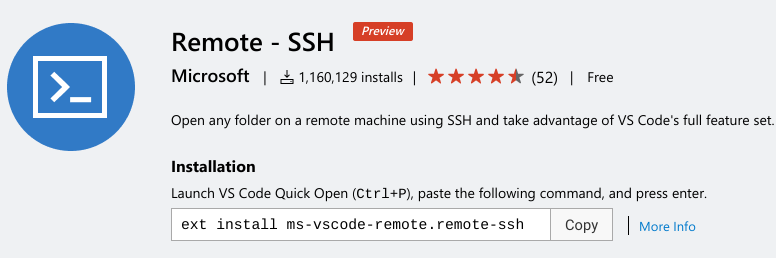
\includegraphics[width=\textwidth]{code-ssh.png}
    \tiny\url{https://marketplace.visualstudio.com/items?itemName=ms-vscode-remote.remote-ssh}
\end{frame}

\begin{frame}
    \centering
    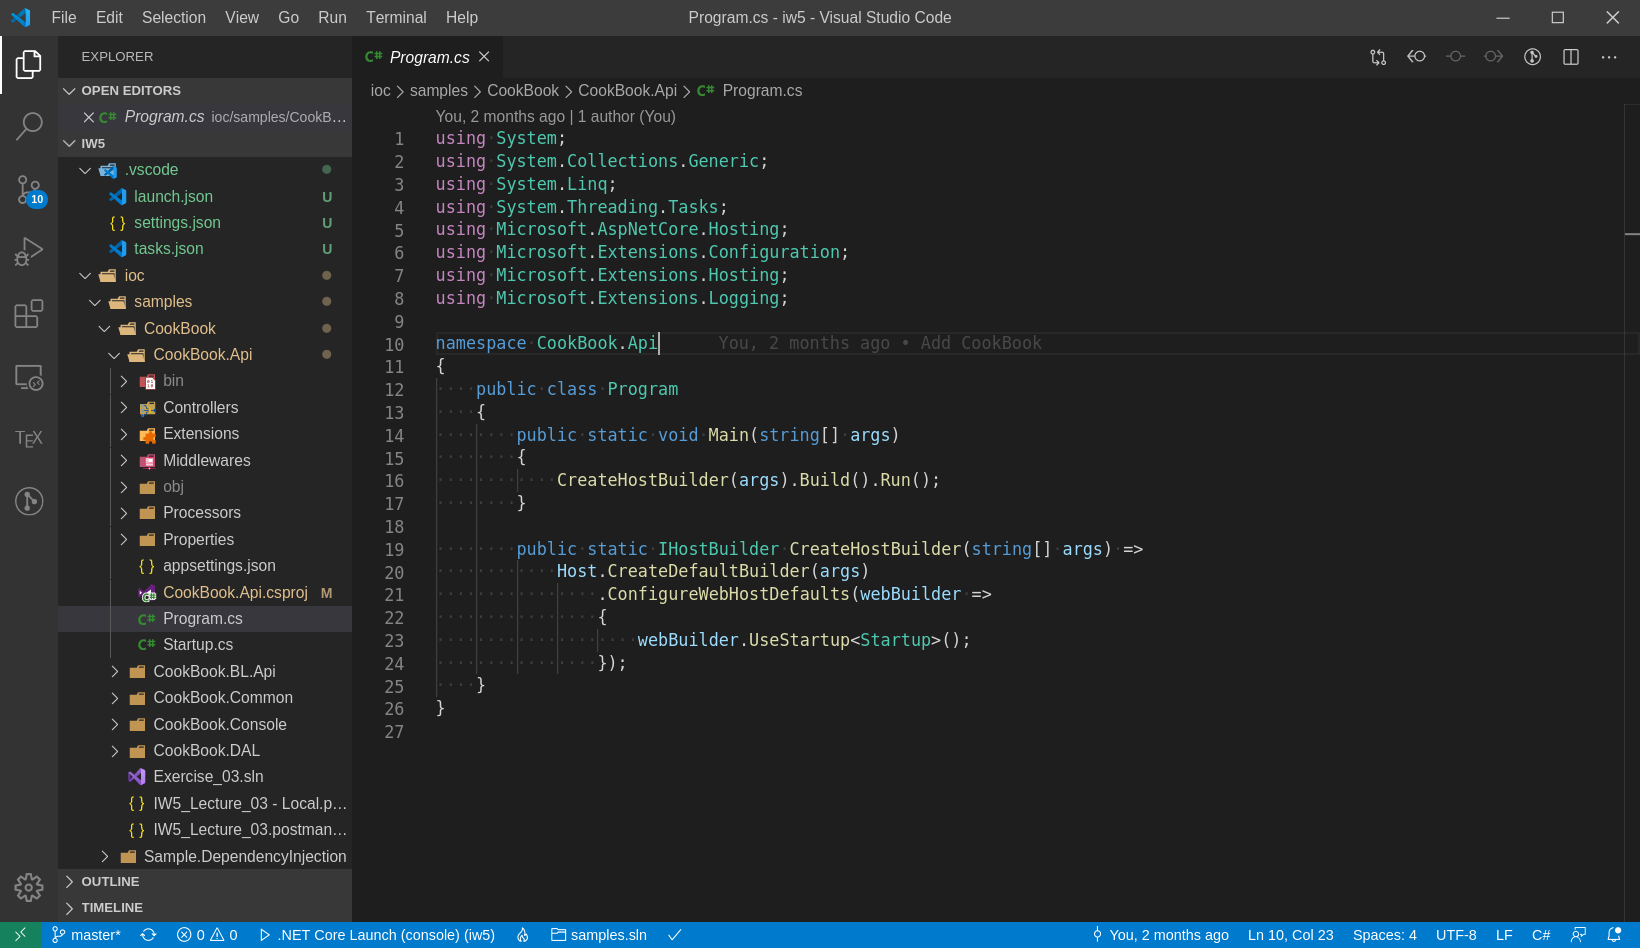
\includegraphics[width=\textwidth]{vscode.png}
    \tiny\url{https://code.visualstudio.com/}
\end{frame}

\begin{frame}
    \centering
    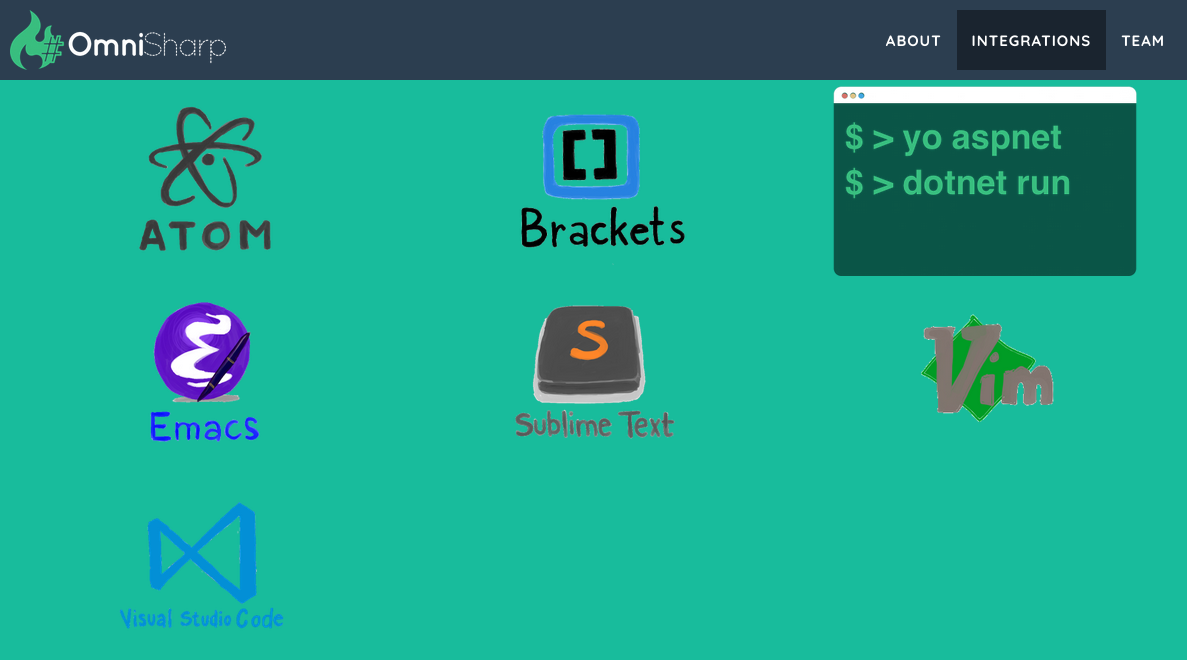
\includegraphics[width=\textwidth]{omnisharp.png}
    \tiny\url{https://www.omnisharp.net}
\end{frame}

\begin{frame}
    \centering
    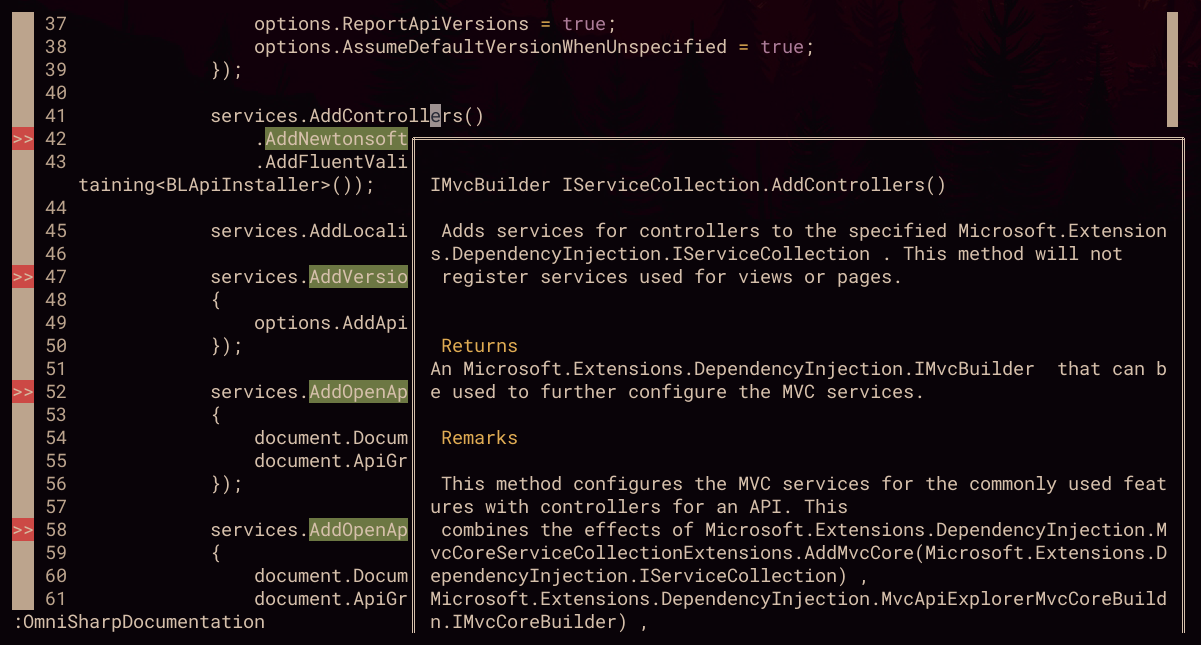
\includegraphics[width=\textwidth]{vim.png}
    \tiny\url{https://github.com/OmniSharp/omnisharp-vim}
\end{frame}

\begin{frame}
    \centering
    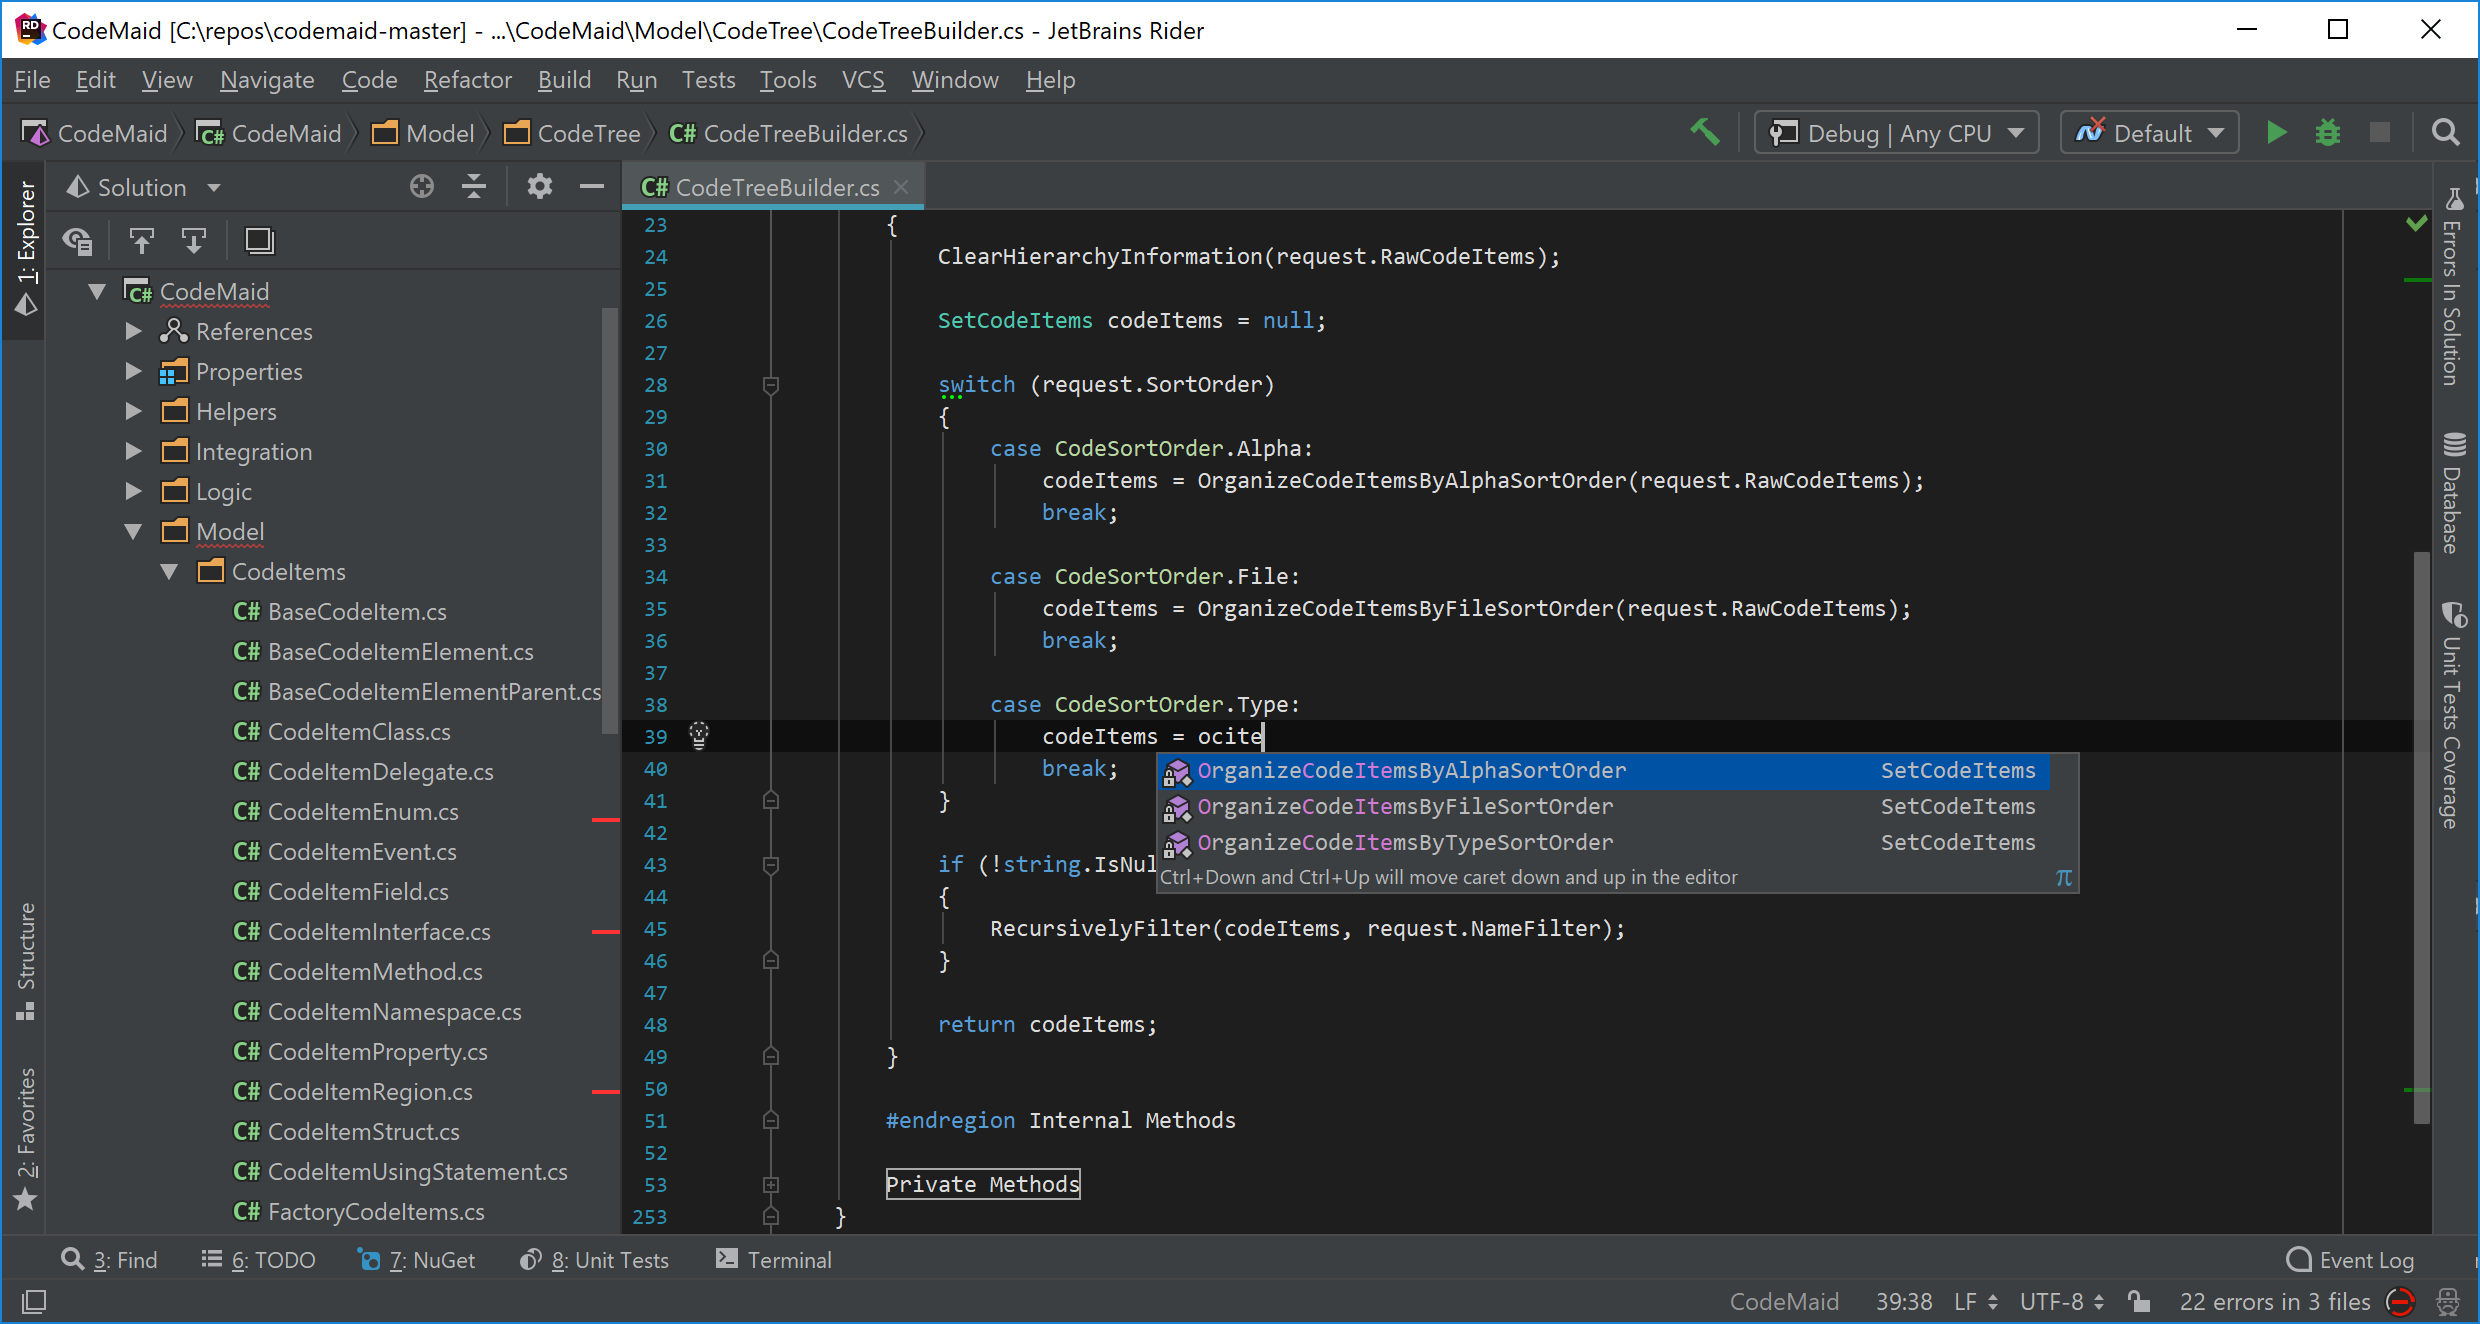
\includegraphics[width=\textwidth]{rider.png}
    \tiny\url{https://www.jetbrains.com/rider}
\end{frame}

\begin{frame}
    \begin{center}
        \Large \texttt{dotnet-sos}
        \\
        \Large \texttt{dotnet-dump}
        \\
        \Large \texttt{dotnet-trace}
        \\
        \vspace{10pt}\tiny\url{https://github.com/dotnet/diagnostics}\\
        \tiny\url{https://www.youtube.com/watch?v=Jw88UYVG9dg}
    \end{center}
\end{frame}

\begin{frame}
    \begin{center}
        \Huge
        \color{vulkan}
        \rmfamily
        \textit{Pauza na čaj}
    \end{center}
\end{frame}

\begin{frame}
    \begin{center}
        \color{vulkan}
        \Huge \textrm{Knihovny}
    \end{center}
\end{frame}

\begin{frame}
    \begin{center}
        \LARGE \textrm{Web}
    \end{center}
\end{frame}

\begin{frame}
    \centering
    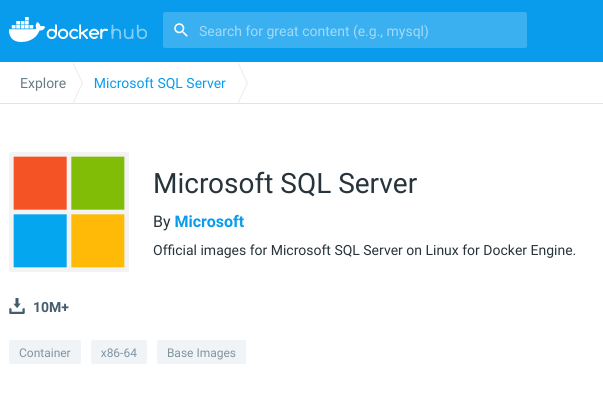
\includegraphics[width=\textwidth]{sqlserver.png}
    \tiny\url{https://hub.docker.com/_/microsoft-mssql-server}
\end{frame}


\begin{frame}
    \begin{center}
        \LARGE \textrm{Terminál}
    \end{center}
\end{frame}

\begin{frame}
    \centering
    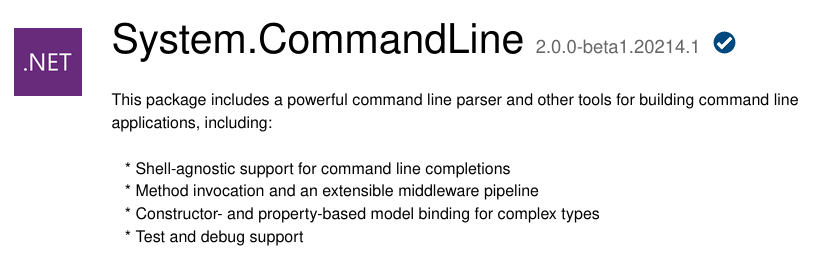
\includegraphics[width=\textwidth]{commandline.png}
    \tiny\url{https://github.com/dotnet/command-line-api}
\end{frame}

\begin{frame}
    \begin{center}
        \ttfamily
        \LARGE
        Sample.Sqrt
    \end{center}
\end{frame}


\begin{frame}
    \begin{center}
        \LARGE \textrm{GUI}
    \end{center}
\end{frame}

\begin{frame}
    \centering
    
\includegraphics[width=\textwidth]{nelectron.png}
    \tiny\url{https://blog.stevensanderson.com/2019/11/01/exploring-lighter-alternatives-to-electron-for-hosting-a-blazor-desktop-app/}
    \tiny\url{https://github.com/ElectronNET/Electron.NET}
\end{frame}

\begin{frame}
    \centering
    
\includegraphics[width=\textwidth]{monogui.png}
    \tiny\url{https://www.mono-project.com/docs/gui/winforms}
    \tiny\url{https://www.mono-project.com/docs/gui/gtksharp/}
    \tiny\url{https://github.com/qmlnet/qmlnet}
    \tiny\url{https://docs.microsoft.com/en-us/xamarin/xamarin-forms/platform/other/gtk}
\end{frame}

\begin{frame}
    \centering
    
\includegraphics[width=\textwidth]{avalonia.png}
    \tiny\url{https://avaloniaui.net/}
\end{frame}

\begin{frame}
    \centering
    
\includegraphics[width=\textwidth]{wine.png}
    \tiny\url{https://ccifra.github.io/PortingWPFAppsToLinux/Overview.html}
\end{frame}


\begin{frame}
    \begin{center}
        \LARGE \textrm{Game Engines}
    \end{center}
\end{frame}

\begin{frame}
    \centering
    
\includegraphics[width=\textwidth]{unity.png}
    \tiny\url{https://unity.com/}
\end{frame}

\begin{frame}
    \centering
    
\includegraphics[width=0.5\textwidth]{monogame.png}
    \\
    \tiny\url{https://www.monogame.net/}
\end{frame}

\begin{frame}
    \centering
    
\includegraphics[width=\textwidth]{godot.png}
    \tiny\url{https://godotengine.org/}
\end{frame}


\begin{frame}
    \begin{center}
        \color{vulkan}
        \Huge \textrm{Problémy}
    \end{center}
\end{frame}

\begin{frame}
    \begin{center}
        \LARGE \textrm{Reference Assemblies}
    \end{center}
\end{frame}

\begin{frame}[fragile]
\begin{center}
\begin{minted}[frame=lines, framesep=5pt]{text}
The reference assemblies for .NETFramework,
Version=v4.7.2 were not found. To resolve this,
install the Developer Pack (SDK/Targeting Pack) for
this framework version or retarget your application.
You can download .NET Framework Developer Packs at
https://aka.ms/msbuild/developerpacks
\end{minted}
\end{center}
\end{frame}

\begin{frame}[fragile]
\begin{center}
\begin{minted}[frame=lines, framesep=5pt]{xml}
<ItemGroup>
  <PackageReference
    Include="Microsoft.NETFramework.ReferenceAssemblies"
    Version="1.0.0"
    PrivateAssets="All" />
</ItemGroup>
\end{minted}
\tiny\url{https://github.com/microsoft/dotnet/tree/master/releases/reference-assemblies}
\end{center}
\end{frame}


\begin{frame}
    \begin{center}
        \LARGE \texttt{.resx}
    \end{center}
\end{frame}

\begin{frame}[fragile]
\begin{center}
\begin{minted}[frame=lines, framesep=5pt]{xml}
<ItemGroup>
  <Compile Update="Resources.Designer.cs">
    <DesignTime>True</DesignTime>
    <AutoGen>True</AutoGen>
    <DependentUpon>Resources.resx</DependentUpon>
  </Compile>
</ItemGroup>
<ItemGroup>
  <EmbeddedResource Update="Resources.resx">
    <Generator>ResXFileCodeGenerator</Generator>
    <LastGenOutput>Resources.Designer.cs</LastGenOutput>
  </EmbeddedResource>
</ItemGroup>
\end{minted}
\end{center}
\end{frame}

\begin{frame}[fragile]
\begin{center}
\begin{minted}[frame=lines, framesep=5pt]{xml}
<ItemGroup>
  <EmbeddedResource Update="Resources.resx">
    <StronglyTypedFileName>Resources.Designer.cs</StronglyTypedFileName>
    <StronglyTypedLanguage>CSharp</StronglyTypedLanguage>
    <StronglyTypedNamespace>Project.Namespace</StronglyTypedNamespace>
    <StronglyTypedClassName>Resources</StronglyTypedClassName>
  </EmbeddedResource>
</ItemGroup>
\end{minted}
\tiny\url{https://github.com/microsoft/msbuild/issues/4751}
\end{center}
\end{frame}


\begin{frame}
    \begin{center}
        \LARGE \textrm{Case}
    \end{center}
\end{frame}

\begin{frame}[fragile]
    \begin{center}
\begin{minted}[frame=lines, framesep=5pt]{sass}
// Modules
@import "Modules/box-wrapper.scss";
@import "Modules/docs-markup";
@import "Modules/grid-view.scss";
@import "Modules/navigation.scss";

// Views
@import "Views/StyleGuide/style-guide.scss";
@import "Views/Public/ErrorSites/error-code.scss";
\end{minted}
    \end{center}
\end{frame}


\begin{frame}
    \begin{center}
        \color{vulkan}
        \Huge \textrm{Jeden .NET}
    \end{center}
\end{frame}

\tale{tale/13.png}
\tale{tale/14.png}
\tale{tale/15.png}

\begin{frame}
    \large
    \ttfamily
    \begin{equation*}
        \texttt{.NET Core 3} + \texttt{.NET Framework 4} + \texttt{Mono 6} = \texttt{.NET 5}
    \end{equation*}
    \\
    \centering
    \tiny\url{https://devblogs.microsoft.com/dotnet/introducing-net-5/}
\end{frame}

\end{document}
